\documentclass[border=5pt, multi, tikz]{standalone}
\definecolor{red}{rgb}{1,.5,.6}
\definecolor{blue}{rgb}{.5,.5,1}

\begin{document}
	
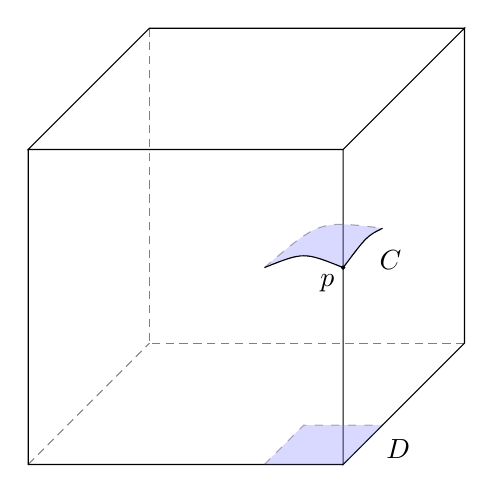
\begin{tikzpicture}
\draw [every edge/.append style={draw=black, densely dashed, opacity=.5}]
(0,0,0) coordinate (o) --
++(-4,0,0) coordinate (a) --
++(0,-4,0) coordinate (b) edge
coordinate [pos=1] (g) ++(0,0,-4) -- ++(4,0,0) coordinate (c) -- cycle
(o) -- ++(0,0,-4) coordinate (d) -- ++(0,-4,0) coordinate (e) edge (g) -- (c) -- cycle
(o) -- (a) -- ++(0,0,-4) coordinate (f) edge (g) -- (d) -- cycle
;
%\draw [fill=blue, opacity=.3, dashed] (-1,-2,0) -- (-.5,-1.5,0) -- (.5,-1.5,0) -- (0,-2,0);

\draw [fill=blue, opacity=.3, dashed] (-1,-4,0) -- (-.5,-3.5,0) -- (.5,-3.5,0) -- (0,-4,0);

\coordinate (x) at (0,-1.5,0);
\coordinate (y) at (-1,-1.5,0);
\coordinate (z) at (.5,-1,0);
% controls
\coordinate (p) at (-.5,-1.3,0);
\coordinate (q) at (-.3,-.9,0);
\coordinate (r) at (.3,-1.1,0);

\draw [fill=blue, opacity=.3, dashed]
(x) .. controls (p) .. 
(y) .. controls (q) ..
(z) .. controls (r) .. (x);

\draw (x) .. controls (p) .. (y);
\draw (z) .. controls (r) .. (x);

\node at (.6,-1.4,0){$C$};
\node at (-.2,-1.7,0){$p$};
\node at (.7,-3.8,0){$D$};
\draw [fill] (x) circle [radius=0.02];
\end{tikzpicture}
\end{document}
















